% задание и сама лабораторная работа
% Для листинга кода:
\lstset{ %
	language=lisp,                 % выбор языка для подсветки (здесь это С++)
	basicstyle=\small\sffamily, % размер и начертание шрифта для подсветки кода
	numbers=left,               % где поставить нумерацию строк (слева\справа)
	numberstyle=\tiny,           % размер шрифта для номеров строк
	stepnumber=1,                   % размер шага между двумя номерами строк
	numbersep=5pt,                % как далеко отстоят номера строк от подсвечиваемого кода
	showspaces=false,            % показывать или нет пробелы специальными отступами
	showstringspaces=false,      % показывать или нет пробелы в строках
	showtabs=false,             % показывать или нет табуляцию в строках
	frame=single,              % рисовать рамку вокруг кода
	tabsize=2,                 % размер табуляции по умолчанию равен 2 пробелам
	captionpos=t,              % позиция заголовка вверху [t] или внизу [b] 
	breaklines=true,           % автоматически переносить строки (да\нет)
	breakatwhitespace=false, % переносить строки только если есть пробел
	escapeinside={\#*}{*)}   % если нужно добавить комментарии в коде
}
\newpage
\section*{Задание}
\addcontentsline{toc}{section}{\tocsecindent{Задание}}

Построить схему выполнения системного вызова open() в зависимости от значения основных флагов определяющих открытие файла на чтение, на запись, на выполнение и на создание нового файла. В схеме должны быть названия функций и кратко указаны выполняемые ими действия. По ГОСТу это делается с помощью выносных линий в фигурных скобках.
В схему нужно обязательно включить следующие действия, выполняемые соответствующими функциями ядра:

1)	копирование названия файла из пространства пользователя в пространство ядра;

2)	блокировка/разблокировка (spinlock) структуры files\_struct и других действий в разных функциях;

3)	алгоритм поиска свободного дескриптора открытого файла;

4)	работу со структурой nameidata – инициализация ее полей;

5)	алгоритм разбора пути (кратко);

6)	инициализацию полей struct file;

7)	«открытие» файла для чтения, записи или выполнения; 

8)	создание inode в случае отсутствия открываемого файла.\\
Отчет должен включать: титульный лист и схему алгоритма работы системного вызова open().
\newpage
\section*{Схема алгоритма}
\addcontentsline{toc}{section}{\tocsecindent{Схема алгоритма}}

\begin{figure}[h!]
	\caption{Схема алгоритма работы системного вызова open()}
	\center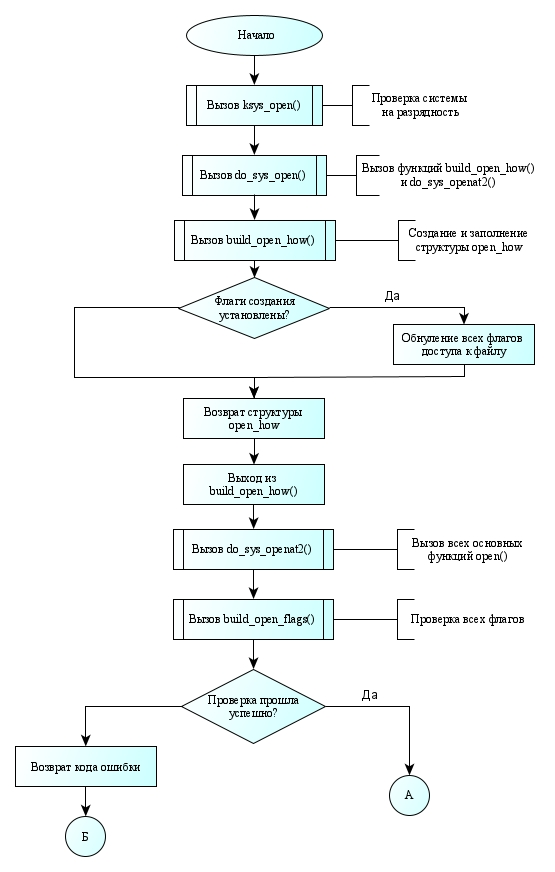
\includegraphics[scale=0.75]{img/1.jpg}
	
\end{figure}
\begin{figure}[h!]
	\caption{Схема алгоритма работы системного вызова open()}
	\center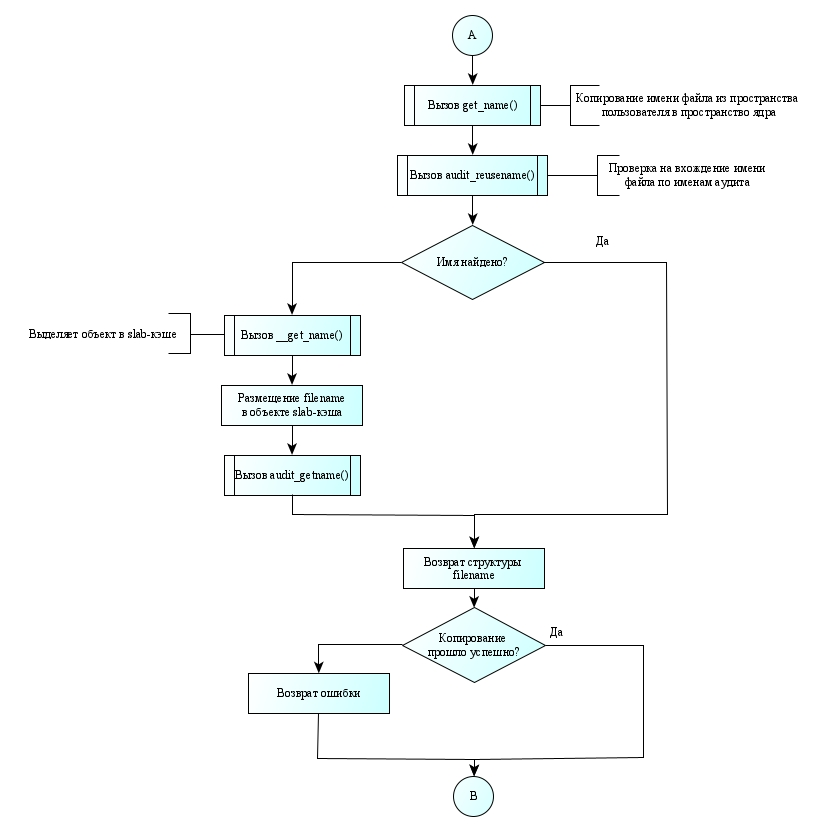
\includegraphics[scale=0.65]{img/2.jpg}
	
\end{figure}

\begin{figure}[h!]
	\caption{Схема алгоритма работы системного вызова open()}
	\center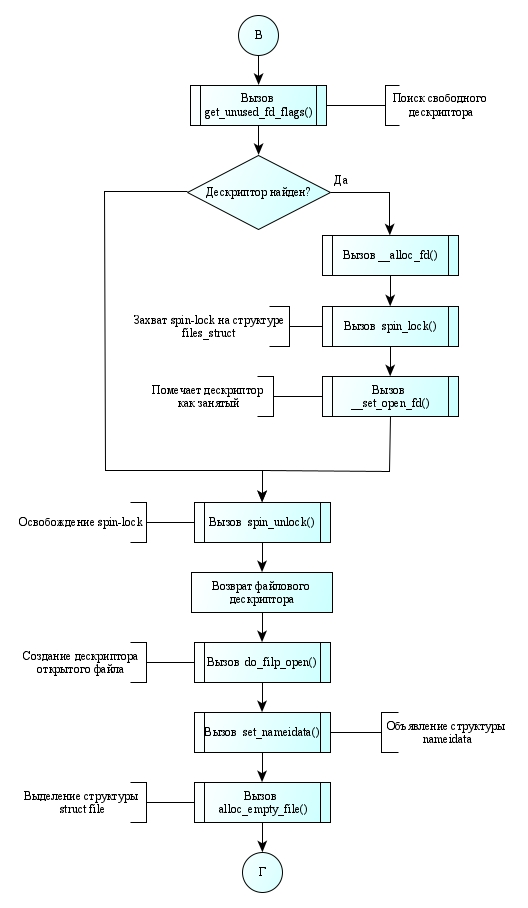
\includegraphics[scale=0.75]{img/3.jpg}
	
\end{figure}
\begin{figure}[h!]
	\caption{Схема алгоритма работы системного вызова open()}
	\center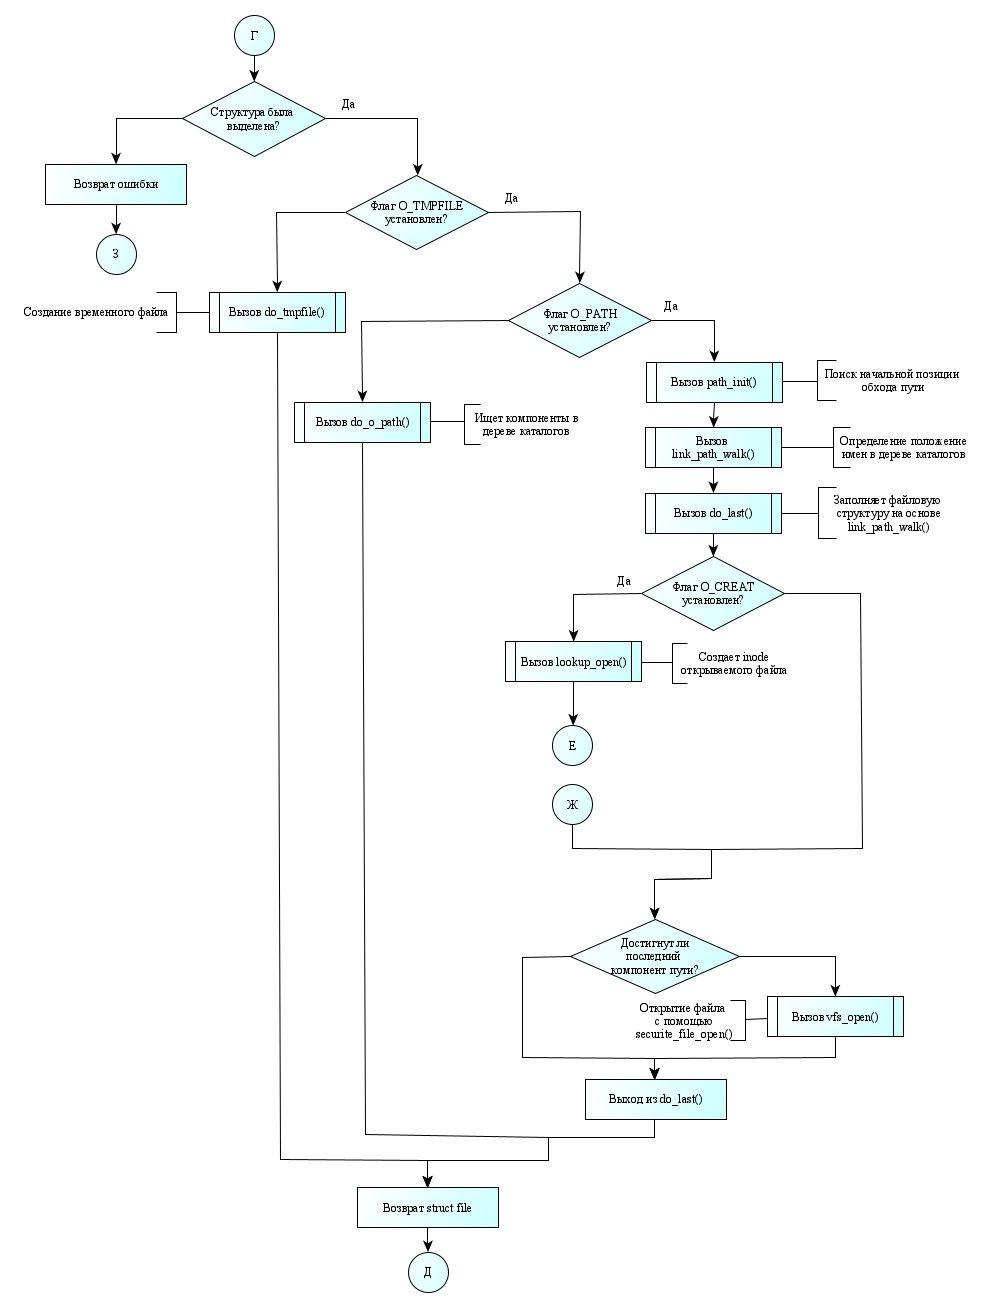
\includegraphics[scale=0.85]{img/4.jpg}
	
\end{figure}
\begin{figure}[h!]
	\caption{Схема алгоритма работы системного вызова open()}
	\center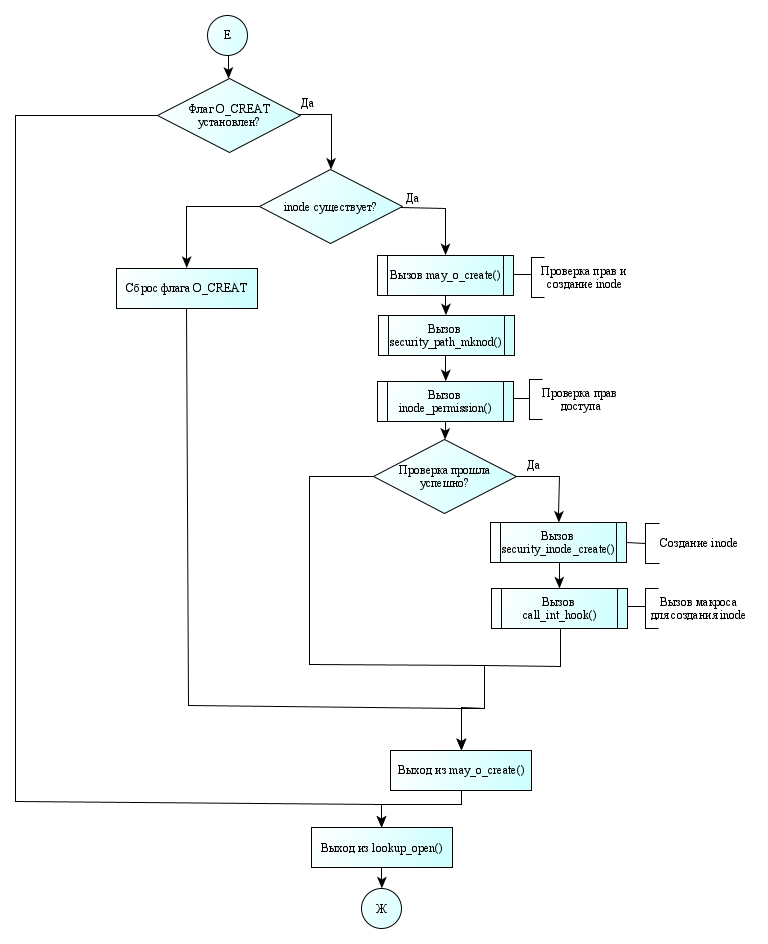
\includegraphics[scale=0.65]{img/41.jpg}
	
\end{figure}
\begin{figure}[h!]
	\caption{Схема алгоритма работы системного вызова open()}
	\center
\includegraphics[scale=0.65]{img/5.jpg}
	
\end{figure}